\begin{answer}{twopiecesofwood}
This is a great question.
Start with the naive approach.
If we measure $a$ and $b$ on their own, we get
\begin{align*}
\E(a)   &= a \\
\Var(a) &= \sigma^2 \\
\E(b)   &= b \\
\Var(b) &= \sigma^2
\end{align*}
We've measured each one with an error of $\sigma^2$.
We can do better.
We can measure the sum of the two sticks, $s = a+b$, and the difference between the two $d = a-b$.
\begin{center}

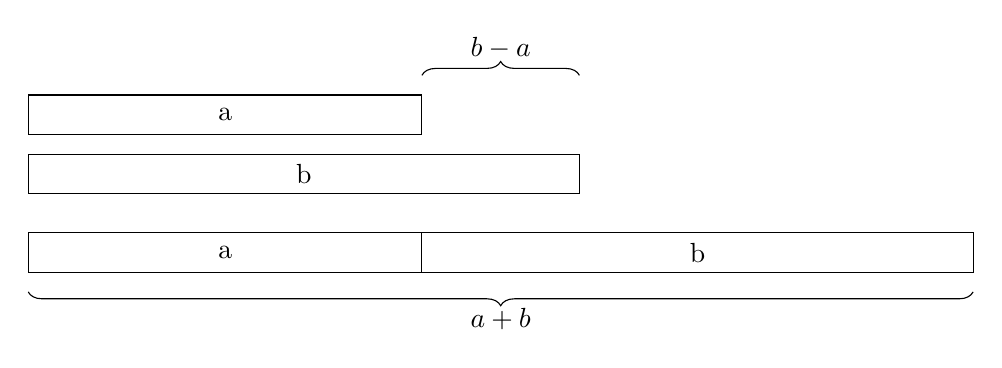
\begin{tikzpicture}
\draw (0,0.75) rectangle ++(5,0.5)node[midway]{a};
\draw (0,0)    rectangle ++(7,0.5) node[midway]{b};
\draw[decorate, decoration={brace, amplitude=5pt}]
      (5,1.5) -- (7,1.5) node (A) [midway, yshift=10pt]{$b-a$};

\draw (0,-1) rectangle ++(5,0.5)node[midway]{a};
\draw (5,-1)    rectangle ++(7,0.5) node[midway]{b};
\draw[decorate, decoration={brace, mirror, amplitude=5pt}]
      (0,-1.25) -- (12,-1.25) node (A) [midway, yshift=-10pt]{$a+b$};
\end{tikzpicture}

\end{center}
Let us solve for $a$ and $b$ in terms of $s$ and $d$, and see what the mean and variance of our estimates are.
\begin{align*}
a   &= \frac{s - d}{2} \\
\E(a)  &= \E\left(\frac{s - d}{2}\right)
        =  a \\
\Var(a) &= \Var\left(\frac{s - d}{2} \right) \\
        &= \frac{1}{4}(\Var(s) + \Var(d)) \\
        &= \frac{1}{2}\sigma^2 \\
        & \quad \text{Likewise, for } b \\
b   &= \frac{s + d}{2} \\
\E(b)  &= \E\left(\frac{s + d}{2}\right)
        =  b \\
\Var(b) &= \Var\left(\frac{s + d}{2} \right) \\
        &= \frac{1}{2}\sigma^2
\end{align*}
What happened here? As if by magic, we were able to reduce our variance by half.
The trick is that we used our tools to measure $a$ and $b$ twice.
Each additional measurement will reduce the variance of our estimator.
\end{answer}
